\section{Discrete Fourier Transform}

\begin{frame}{Complex Numbers Review}
  \begin{columns}
    \begin{column}{0.65\textwidth}
      \begin{itemize}
        \item The \emph{complex numbers} are pairs of real numbers
        \item with \emph{Real} and {Complex Parts}
        \item Visualize on the \emph{Complex Plane}
        \item and analogize to a 2-d vector with the L-2 norm
        \item Write in two forms:
        \begin{itemize}
          \item $a + bj$ (Cartesian)
          \item $\alpha \exp(j \phi)$ (polar)
        \end{itemize}
        and relate using Euler's formula
        \begin{equation}
          \alpha \exp(j \phi) = \alpha \cos(\phi) + j \alpha \sin(\phi)
        \end{equation}
      \end{itemize}
    \end{column}
    \begin{column}{0.35\textwidth}
      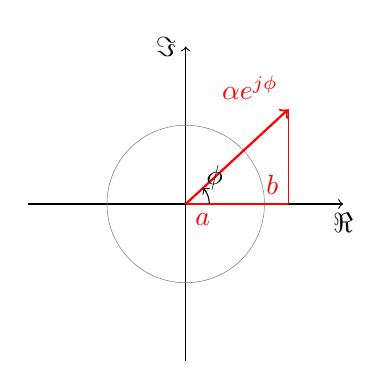
\begin{tikzpicture}
        \draw[->] (-2,0) -- (2,0) node[below] {$\Re$};
        \draw[->] (0,-2) -- (0,2) node[left] {$\Im$};
        \draw[help lines] (0,0) circle (1);

        \draw [->,red,thick] (0,0) -- (1.3,1.2) node [above left] {$\alpha e^{j \phi} $};
        \draw [red] (1.3,1.2) -- (1.3,0) node [above left] {$b$};
        \draw [red] (1.3,0) -- (0,0) node [below right] {$a$};

        \draw[->] (0:.3) arc (0:42.71:.3);
        \node at (42.71:.5) {$\phi$};
      \end{tikzpicture}
    \end{column}
  \end{columns}
\end{frame}

\begin{frame}{More Useful Formulae}
  \begin{itemize}
    \item Sinusoids to complex exponentials:
    \begin{equation}
      \cos(x) = \frac{e^{jx}+e^{-jx}}{2}
    \end{equation}
    \begin{equation}
      \sin(x) = \frac{e^{jx}-e^{-jx}}{2j}
    \end{equation}
  \item Complex Inner Product:
    \begin{equation*}
      \innerproduct{x}{y} = y^* x
    \end{equation*}
    \begin{equation*}
      \norm{x}_2^2 = \innerproduct{x}{x} 
    \end{equation*}
  \end{itemize}
\end{frame}

\begin{frame}{Roots of Unity}
  \def\n{5}
  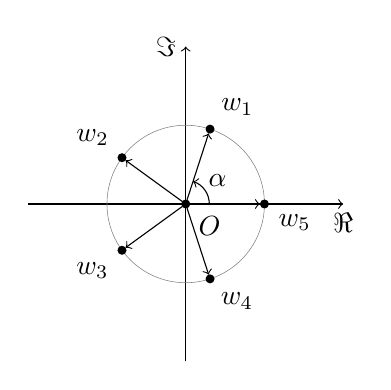
\begin{tikzpicture}[
  dot/.style={draw,fill,circle,inner sep=1pt}
  ]
  \draw[->] (-2,0) -- (2,0) node[below] {$\Re$};
  \draw[->] (0,-2) -- (0,2) node[left] {$\Im$};
  \draw[help lines] (0,0) circle (1);

  \node[dot,label={below right:$O$}] (O) at (0,0) {};
  \foreach \i in {1,...,\n} {
    \node[dot,label={\i*360/\n-(\i==\n)*45:$w_{\i}$}] (w\i) at (\i*360/\n:1) {};
    \draw[->] (O) -- (w\i);
  }
  \draw[->] (0:.3) arc (0:360/\n:.3);
  \node at (360/\n/2:.5) {$\alpha$};
\end{tikzpicture}
\end{frame}

\begin{frame}{Roots of Unity}
  \begin{itemize}
    \item \vocab{N\textsuperscript{th} root of unity} $\omega_N$ is defined to satisfy
      \begin{equation*}
        (\omega_N)^N = 1
      \end{equation*}
    \item $N$ numbers sweeping around the complex unit circle satisfy this:
      \begin{equation*}
        \omega_{k,N} = e^{j \frac{2 \pi k}{N}}
      \end{equation*}
    \item Noting that the $k$ can be pulled out of the exponent, this can also be written
      \begin{equation*}
        \omega_N^k
      \end{equation*}
  \end{itemize}
\end{frame}

